\documentclass{beamer}

\usetheme{metropolis}
\definecolor{mediumred}{RGB}{180, 10, 5}
\setbeamercolor{frametitle}{bg=mediumred, fg=white}

\usepackage{tkz-graph}
\usepackage{tikz}
\usetikzlibrary{arrows,matrix,decorations.pathreplacing,positioning,chains,fit,shapes,calc} %
\usetikzlibrary{calc,patterns,decorations.pathmorphing,decorations.markings}

\usepackage{siunitx}
\usepackage{minted}

\usepackage{../../latex/custom}

\newcommand{\expe}[2]{\la #1, #2 \ra}

\newcommand\Wider[2][3em]{%
\makebox[\linewidth][c]{%
  \begin{minipage}{\dimexpr\textwidth+#1\relax}
  \raggedright#2
  \end{minipage}%
  }%
}

\title{Computing polynomial controlled invariant sets using Sum-of-Squares Programming}
\date{}
\author{Beno\^it Legat${}^*$, \emph{In collaboration with}: Rapha\"el M. Jungers${}^*$ and Paulo Tabuada${}^\dagger$}
\institute{${}^*$ UCLouvain, ${}^\dagger$ UCLA}

\makeatletter
\let\@@magyar@captionfix\relax
\makeatother

\begin{document}
\maketitle

\begin{frame}{Information Theory}
  \includegraphics[width=0.33\textwidth]{tetra0pm.png}~%
  \includegraphics[width=0.33\textwidth]{tetra0zy.png}~%
  \includegraphics[trim=6cm 2cm 6cm 7cm,clip,width=0.33\textheight]{tetra0bound15789.png}

  See presentation at \emph{37rd Symposium on Information Theory in the Benelux}, 2016.
\end{frame}

\begin{frame}{Safe Model Predictive Control}
  \begin{center}
    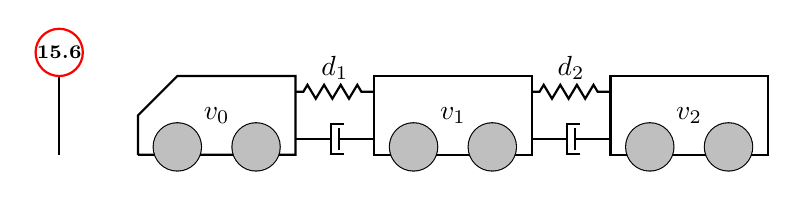
\begin{tikzpicture}
      \tikzstyle{spring}=[thick,decorate,decoration={zigzag,pre length=0.1cm,post length=0.1cm,segment length=6}]
\tikzstyle{damper}=[thick,decoration={markings,
  mark connection node=dmp,
  mark=at position 0.5 with
  {
    \node (dmp) [thick,inner sep=0pt,transform shape,rotate=-90,minimum width=10pt,minimum height=2pt,draw=none] {};
    \draw [thick] ($(dmp.north east)+(2pt,0)$) -- (dmp.south east) -- (dmp.south west) -- ($(dmp.north west)+(2pt,0)$);
    \draw [thick] ($(dmp.north)+(0,-4pt)$) -- ($(dmp.north)+(0,4pt)$);
  }
}, decorate]
\draw[thick] (0, 0) -- (2, 0) -- (2, 1) -- (0.5, 1) -- (0, 0.5) -- (0, 0);
\draw [spring] (2, 0.8) -- (3, 0.8);
\draw [damper] (2, 0.2) -- (3, 0.2);
\draw[thick] (3, 0) rectangle (5, 1);
\draw [spring] (5, 0.8) -- (6, 0.8);
\draw [damper] (5, 0.2) -- (6, 0.2);
\draw[thick] (6, 0) rectangle (8, 1);
\draw[thick] (0.5, 0.1) circle (0.3);
\fill[color=lightgray] (0.5, 0.1) circle (0.3);
\draw[thick] (1.5, 0.1) circle (0.3);
\fill[color=lightgray] (1.5, 0.1) circle (0.3);
\draw[thick] (3.5, 0.1) circle (0.3);
\fill[color=lightgray] (3.5, 0.1) circle (0.3);
\draw[thick] (4.5, 0.1) circle (0.3);
\fill[color=lightgray] (4.5, 0.1) circle (0.3);
\draw[thick] (6.5, 0.1) circle (0.3);
\fill[color=lightgray] (6.5, 0.1) circle (0.3);
\draw[thick] (7.5, 0.1) circle (0.3);
\fill[color=lightgray] (7.5, 0.1) circle (0.3);
\node at (1, 0.5) {$v_0$};
\node at (4, 0.5) {$v_1$};
\node at (7, 0.5) {$v_2$};
\node at (2.5, 1.1) {$d_1$};
\node at (5.5, 1.1) {$d_2$};

      \draw[thick] (-1, 0) to (-1, 1);
      \draw[thick,color=red] (-1, 1.3) circle (0.3);
      \node at (-1, 1.3) {\scriptsize \bf 15.6};
    \end{tikzpicture}

    \includegraphics[width=0.45\textwidth]{CruiseControlSets_d_u.png}
    ~
    \includegraphics[width=0.45\textwidth]{CruiseControlSets_v0_u.png}
  \end{center}

  See presentation at \emph{IFAC Conference on Analysis and Design of Hybrid Systems} (ADHS), 2018.
\end{frame}

\begin{frame}{Safe Stochastic Programming}
  \begin{center}
    \includegraphics[width=0.4\textwidth]{reservoir.jpg}~%
    \includegraphics[trim=.2cm .2cm .2cm .2cm, clip, width=0.6\textwidth]{ReservoirEllipsoidal.pdf}
  \end{center}
  See presentation at \emph{23rd International Symposium on Mathematical Programming} (ISMP), 2018.
\end{frame}

\begin{frame}[fragile]
  \frametitle{Running example}
  Consider control system:
  \begin{align*}
  v_{k+1} & = v_k + a_k \Delta t\\
  a_{k+1} & = u_k
  \end{align*}

  The system is $x_{k+1} = Ax_k + Bu_k$ where
  $$
  A = \begin{bmatrix}
  1 & \Delta t\\
  0 & 0
  \end{bmatrix}, \qquad
  B = \begin{bmatrix}
  0\\
  1
  \end{bmatrix}.
  $$

  As we will see, a set $S$ is controlled invariant iff
  $$
  \begin{bmatrix}
  1 & \Delta t
  \end{bmatrix}
  S \subseteq
  \begin{bmatrix}
  1 & 0
  \end{bmatrix}
  S
  $$
\end{frame}

\begin{frame}{Controlled invariant set}
  \begin{block}{Linear discrete control system}
    \[ x_{k+1} = A x_k + B u_k, \quad x_k \in X, u_k \in U \]
  \end{block}
  \begin{block}{Controlled invariant set}
    Set $S \subseteq X$ \emph{controlled invariant} iff
    \[ \forall x \in S, \exists u \in U \text{ such that } Ax + Bu \in S \]
  \end{block}
\end{frame}

\begin{frame}{Unconstrained input without loss of generality}
  \begin{block}{\alert{Constrained} input}
    \[ x_{k+1} = A x_k + B u_k, \quad x_k \in X, \alert{u_k \in U} \]
  \end{block}
  \textbf{\alert{Lift} to \alert{un}constrained input}: $x' = (x, u)$
  \begin{align*}
    x_{k+1} & =
    \begin{pmatrix}
      A & B
    \end{pmatrix}
    x'_k\\
    u_{k+1} & =
    u'_k
  \end{align*}
  where $x'_k \in X' = X \times U$.
\end{frame}


\begin{frame}{Unconstrained control to algebraic system}
  \begin{block}{Linear Discrete \alert{Control} System (DT\alert{C}S)}
    \[ x_{k+1} = A x_k + B u_k, \quad x_k \in X \]
  \end{block}
  \begin{block}{Linear Discrete \alert{Algebraic} System (DT\alert{A}S)}
    \[ Ex_{k+1} = A x_k, \quad x_k \in X \]
    Invariant Set $S \subseteq X$ if
    \[ \forall x \in S, \alert{\exists} y \in S : Ey = Ax \]
  \end{block}
  \begin{block}{Reduction}
    The set $S$ is controlled invariant for the DT\alert{C}S iff
    it is invariant for the DT\alert{A}S
    \[ \Pi x_{k+1} = \Pi A x_k, \quad x_k \in X \]
    where $\Pi$ is a projection on $\Image(B)^\perp$.
  \end{block}
\end{frame}


\begin{frame}{Ellipsoidal controlled invariant Set of Algebraic Systems}
  \[ E x_{k+1} = A x_k, \quad x_k \in X \]
  Convex set $S$ invariant iff
  \begin{align*}
    AS & \subseteq ES\\
    (AS)^\circ & \supseteq (ES)^\circ\\
    A^{-\Tr}S^\circ & \supseteq E^{-\Tr}S^\circ
  \end{align*}
  \begin{block}{Ellipsoidal computation}
    \[ C^\circ = \{\, x \mid x^\Tr Q x \le 1 \,\} \quad \Rightarrow \quad A^{-\Tr}C^\circ = \{\, x \mid x^\Tr A Q A^\Tr x \le 1 \,\} \]
    S-procedure:
    \[ E Q E^\Tr - A Q A^\Tr \text{ is PSD}. \]
  \end{block}
\end{frame}


\begin{frame}[fragile]
  \frametitle{Example with ellipsoids: Model}
  Maximal volume ellipsoid (determinant):
  \begin{center}
    \includegraphics[width=\textwidth]{SetProg_Ellipsoid_AE.png}
  \end{center}
  Maximal sum of the squares of the semi-axes of the ellipsoid (trace):
  \begin{minted}{julia}
@objective(model, Max,
           L1_heuristic(volume(S), [1.0, 1.0]))
  \end{minted}
\end{frame}

\begin{frame}{Example with ellipsoids: Primal Solution}
  \begin{center}
    \includegraphics[width=0.95\textwidth]{SimpleControlledInvariantEllipsoid.png}~%
  \end{center}
  {\scriptsize Maximal volume (blue) and maximal sum of the squares of the semi-axes (red).}
\end{frame}
\begin{frame}{Example with ellipsoids: Polar Solution}
  \begin{center}
    \includegraphics[width=0.95\textwidth]{SimpleControlledInvariantPolarEllipsoid.png}
  \end{center}
  {\scriptsize Maximal volume (blue) and maximal sum of the squares of the semi-axes (red).}
\end{frame}


\begin{frame}{Support function vs polar set}
  \begin{center}
    \includegraphics[width=\textwidth]{support_function_polar.png}
  \end{center}
  Hiriart-Urruty, Lemaréchal, \emph{Fundamentals of convex analysis}, \textbf{2001}.
\end{frame}

\begin{frame}{Support function interpretation}
  Support function:
  \[ \supfun{y}{\Csetvar} = \sup_{x \in \Csetvar} \la y, x \ra. \]
  Key property:
  \[ \supfun{y}{A\Csetvar} = \supfun{A^\Tr y}{\Csetvar}. \]

  \begin{align*}
    AS & \subseteq ES\\
    \supfun{y}{AS} & \le \supfun{y}{ES} & \forall y\\
    \supfun{A^\Tr y}{S} & \le \supfun{E^\Tr y}{S} & \forall y
  \end{align*}

  \begin{block}{Ellipsoidal computation}
    \[ \supfun{y}{C} = \sqrt{x^\Tr Q x} \]
  \end{block}
\end{frame}

\begin{frame}{Polynomial support function}
  Polynomial $p(x)$, e.g. $p(x) = x^4 + y^4$.

  \begin{block}{Polar interpretation}
    \[ C^\circ = \{\, x \mid p(x) \le 1 \,\}. \]
  \end{block}

  \begin{block}{Support function interpretation}
    \[ \supfun{y}{C} = p(x)^{\frac{1}{2d}}. \]
  \end{block}
\end{frame}

\begin{frame}[fragile]
  \frametitle{Example with polynomial sublevel set: Model}
  \begin{minted}{julia}
@variable(model, S, PolySet(degree=d, convex=true,
                            symmetric=true))
  \end{minted}
  Use L1 norm as volume heuristic.

  Convexity ensured by Sum-of-Squares convexity, i.e.,
  $y^\Tr \Hess(x) y$ is Sum-of-Squares for all $x, y$.
\end{frame}

\begin{frame}{Example with polynomial sublevel set: Primal Solution}
  \begin{center}
    \includegraphics[width=0.95\textwidth]{SimpleControlledInvariantPolySet.png}
  \end{center}
  {\footnotesize Degree 4 (orange), 8 (blue), 18 (green) and 22 (red).}
\end{frame}
\begin{frame}{Example with polynomial sublevel set: Polar Solution}
  \begin{center}
    \includegraphics[width=0.95\textwidth]{SimpleControlledInvariantPolarPolySet.png}~%
  \end{center}
  {\footnotesize Degree 4 (orange), 8 (blue), 18 (green) and 22 (red).}
\end{frame}

\begin{frame}
  \frametitle{Exposed face}
  \emph{Exposed face} of convex set $\Csetvar$ associated to $y$ is:
  \[
    F_\Csetvar(y) = \{\, x \in \Csetvar \mid \la x, y \ra = \supfun{y}{\Csetvar} \,\}.
  \]
  \begin{center}
    \includegraphics[width=\textwidth]{faces.png}
  \end{center}
  Vera Roshchina, \emph{Faces of convex sets}.
\end{frame}


\begin{frame}{Continuous time}
  Continuous-time \alert{control} system:
  \begin{equation}
    \label{eq:cs}
    \dot{x} = Ax + Bu
  \end{equation}
  Continuous-time \alert{algebraic} system, $E, A \in \mathbb{R}^{r \times n}$:
  \begin{equation}
    \label{eq:as}
    E\dot{x} = Ax.
  \end{equation}

  \alert{Convex} set invariant iff:
  \[
    \forall z \in \mathbb{R}^r, \forall x \in F_\Csetvar(E^\Tr z), \la z, Ax \ra \le 0.
  \]
\end{frame}

\begin{frame}{Polyhedral controlled invariant set}
  Suppose $r = 1$, $F_\Csetvar(E^\Tr \cdot [-1]) = \{x_1\}$, $F_\Csetvar(E^\Tr \cdot [-1]) = \{x_2\}$,
  Square invariant iff
  \begin{align*}
    Ax_1 & \le 0 & Ax_2 & \ge 0.
  \end{align*}
  \begin{center}
    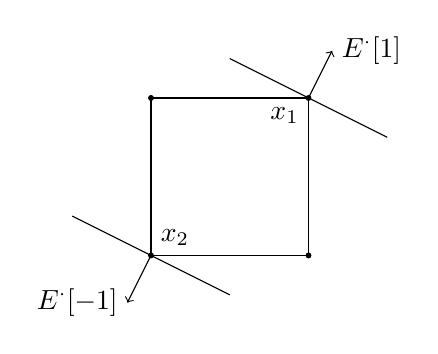
\begin{tikzpicture}
      \draw (1, 1) -- (1, -1) -- (-1, -1) -- (-1, 1) -- (1, 1);
      \draw[fill] ( 1,  1) circle(0.03);
      \draw[fill] ( 1, -1) circle(0.03);
      \draw[fill] (-1,  1) circle(0.03);
      \draw[fill] (-1, -1) circle(0.03);
      \draw (0, 1.5) -- (2, 0.5);
      \draw (0, -1.5) -- (-2, -0.5);
      \draw[->] (1, 1) -- (1.3, 1.6);
      \draw[->] (-1, -1) -- (-1.3, -1.6);
      \node[right] at (1.3, 1.6) {$E^\Tr \cdot [1]$};
      \node[left] at (-1.3, -1.6) {$E^\Tr \cdot [-1]$};
      \node[below left] at (1, 1) {$x_1$};
      \node[above right] at (-1, -1) {$x_2$};
    \end{tikzpicture}
  \end{center}
\end{frame}

\begin{frame}{Polynomial support function}
  If $\supfun{\cdot}{\Csetvar}$ is \alert{differentiable}:
  \[
    \forall z \in \mathbb{R}^r, \la z, A \grad \supfun{E^\Tr z}{\Csetvar} \ra \le 0.
  \]

  If $\supfun{y}{\Csetvar} = \sqrt{y^\Tr P y}$, $\Csetvar$ controlled invariant iff
  \[
    AP^{-1}E^\Tr + EP^{-1}A^\Tr \preceq 0.
  \]

  If $\supfun{y}{\Csetvar} = p(y)^{\frac{1}{2d}}$, then
  \[
    \grad \supfun{y}{\Csetvar} = \frac{1}{p(y)^{1-\frac{1}{2d}}} \grad p(y)
  \]
  and $\Csetvar$ controlled invariant iff
  \[
    z^\Tr A \grad p(E^\Tr z) \le 0 \qquad \forall z \in \mathbb{R}^r.
  \]
\end{frame}

\begin{frame}{Conclusion}
  \begin{itemize}
    \item Controlled invariance condition based on \alert{support function}.
    \item \alert{Semidefinite} program for quadratic support function.
    \item \alert{Sum-of-Squares} program for polynomial support function of arbitrary degree.
    \item Compute invariant sets with the \jlpkg{SetProg} and  \jlpkg{SumOfSquares} extensions of \jlpkg{JuMP} (stickers available)
  \end{itemize}
  \begin{center}
    \includegraphics[width=0.5\textwidth]{JuMP.png}
  \end{center}
\end{frame}

\end{document}
